% 2019-03-06

\documentclass[10pt]{article}
\usepackage[T1]{fontenc}
\usepackage{amssymb}
\usepackage{amsmath}
\usepackage{graphicx}
% \begin{figure}[h]
% \centering
% \includegraphics[width=6.5in]{folder/photo.png}
% \caption{}
% \label{}
% \end{figure}



\usepackage{tikz}
\usetikzlibrary{arrows}
\usepackage{subfigure}
\usepackage{stackrel}
\usepackage{blindtext}

\usepackage[url=false]{biblatex}
\addbibresource{library.bib}

\oddsidemargin=0.15in
\evensidemargin=0.15in
\topmargin=-.5in
\textheight=9in
\textwidth=6.25in

\usepackage[colorlinks=true,breaklinks,pdfpagemode=none,linkcolor=blue,citecolor=blue]{hyperref}

\usepackage{enumerate}
% \vspace{-6pt}
% \begin{itemize}
%     \setlength{\itemsep}{0pt}%
%     \setlength{\parskip}{0pt}%
%     \item Item 1
%     \item Item 2
%         \begin{itemize}
%             \setlength{\itemsep}{0pt}%
%             \setlength{\parskip}{0pt}%
%             \item Sublist Item 1
%             \item Sublist Item 2
%         \end{itemize}
%         \item Item 3
% \end{itemize}
% \vspace{-6pt}


\usepackage{enumitem}
\setlist{itemsep=0mm}

\usepackage{amsmath,amsfonts,amssymb,bm}

\usepackage{scrextend}

\begin{document}

   \noindent
   \begin{center}

   \hrulefill
   
   \vspace{5pt}
   
   \makebox[\textwidth]{ {\bf Energy Systems Analysis} \hfill  A.D. Smith 2019}
   \vspace{0pt}
   
   {\Large \hfill  Lecture 21.  
Power Generation at Utility Scale}
% (Location and Timing)
   \vspace{5pt}
   
  
   \hrulefill
   \end{center}

{\color{darkgray}{\center{ \small{      ``Nobody knew what electricity was until long after Edison's first grid was built and had burned down \ldots [yet] it was uniquely capable of powering things at a distance and doing so very close to instantaneously.''
\\%[3pt]
\rightline{{\rm --- Gretchen Bakke \cite{bakke}}}}}}}

\section{Electricity Market Basics}

Hopefully you remember from Lecture 3 that there are a few key divisions within the electricity sector. The entities involved in the operations of the power grid as a whole can be grouped as follows:

\vspace{-6pt}
\begin{itemize}
    \setlength{\itemsep}{0pt}%
    \setlength{\parskip}{0pt}%
    \item Generators
    \item Transmission system
    \item Distribution system
    \item End users
\end{itemize}
\vspace{-6pt}

Unless we're talking about distributed generation (and we will in the next lecture), the end user is usually far away from the generator. Also, an individual building typically needs only a tiny fraction of the power being produced at a power plant. Therefore, the two steps in the middle (transmission and distribution) are about getting power to a consumer to a group of consumers that are spatially separated (point-to-area flows \cite{Bejan2017-ff}), and along the way stepping down that power to an appropriate voltage for the consumers (resulting in fast travel over longer distances and slower travel over shorter distances \cite{Bejan2017-ff}). 

Figs. \ref{eiaill} and \ref{ucsill} illustrate the basics of the current system architecture.

\medskip
            \begin{figure}[h]
            \centering
            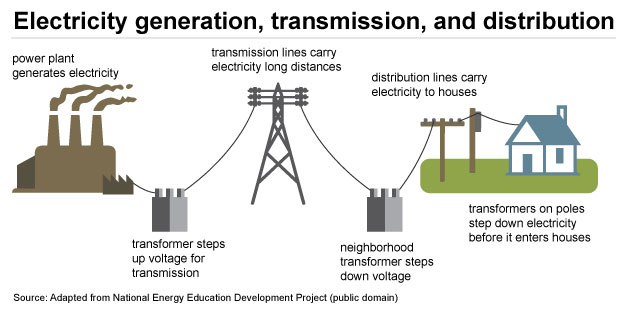
\includegraphics[width=12cm]{extras21/transmission.jpg}
            \caption{Electricity generation, transmission, and distribution basics \cite{howelectricity}}
            \label{eiaill}
            \end{figure}
\bigskip

\medskip
            \begin{figure}[h]
            \centering
            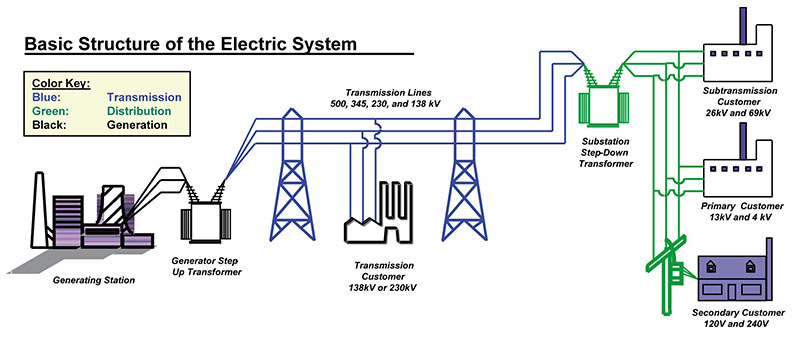
\includegraphics[width=12cm]{extras21/ucsill.jpg}
            \caption{Basic Structure of the Electric System \cite{howtheelectricity}}
            \label{ucsill}
            \end{figure}
\bigskip

Here on campus, most of our electricity demand is served by our local utility, and a small fraction of campus demand is met by electricity produced from our turbine power generation and hot water facility, a combined heat and power system (discussed in Lecture 22). Rocky Mountain Power (RMP) (a division of PacifiCorp utility company, which is itself a subsidiary of Berkshire Hathaway Energy) is a vertically integrated, regulated \cite{noauthor_undated-eo} utility company. %That means . 
They cover most of Utah (Fig. \ref{rmp}), and the small independent power districts (such as the municipal systems of Murray or Provo) still interact with them through, for example, purchasing electricity from RMP generators or paying to use their transmission services. 

The region of the power grid that we belong to is called the Western Interconnect or simply the western grid. It includes Rocky Mountain Power's service area, as well as others including California---a large and complex system extending throughout the Rocky Mountains and encompassing all of the U.S. that is west of it, as illustrated in Fig. \ref{grid}.

\medskip
            \begin{figure}[h]
            \centering
            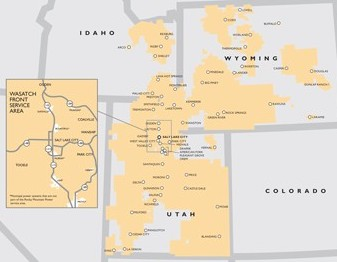
\includegraphics[width=9cm]{extras21/servicearea.jpg}
            \caption{Rocky Mountain Power Service Area \cite{servicearea}}
            \label{rmp}
            \end{figure}


            \begin{figure}[h]
            \centering
            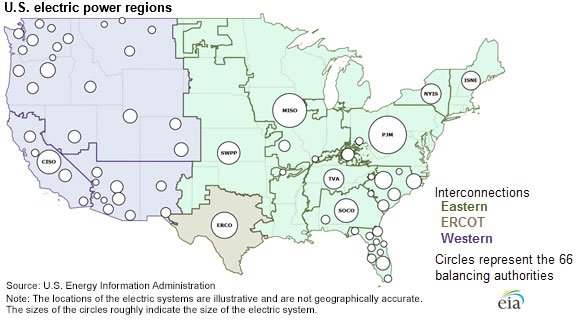
\includegraphics[width=13.5cm]{extras21/elect_power_regions.jpg}
            \caption{U.S. Electric Power Regions  \cite{howelectricity}}
            \label{grid}
            \end{figure}



\section{Timing of Power Generation and Power Consumption%, \& valuation
}

Because the load that the generators on the grid are trying to meet is not constant over time, and neither is the set of available generators, the value of energy varies over time. We have historically been billed per kWh because it is only relatively recently in the history of the grid that the metering technology has existed to keep track of \textit{when} electricity is being delivered (as opposed to how much). To get a look at how electricity demand (and, therefore, production) are varying in real time, take a moment and look at the California Independent System Operator (CAISO) website called ``Today's Outlook'' at \url{http://www.caiso.com/TodaysOutlook/Pages/default.aspx} and view today's demand trend profile (illustrating forecasted and actual demand so far today). California ISO is a large independent grid operator providing a great deal of information about the system they manage \cite{CAISO}. You can also find their real-time data app ``ISO Today'' in the app store for either Apple or Google Play.

% So what did you think about the size of the load and the accuracy of the load predictions at different time intervals?

% How about putting the demand in context:
% ``roughly enough electricity for the instantaneous demand of 750 homes at once.'' \cite{understandingelectricity}
% Now, are you surprised at how large or small the load is in this region covering most of the state of California (and a bit of Nevada)?

% Speaking of that, let's define demand and make sure we're on the same page \ldots

\section{Power Generation Terminology}

These are key terms that will lay the foundation for our further discussions on comparing options for power generation, economic analysis and primary energy analysis.

\begin{labeling}{longest item in list long}

\item [\textbf{capacity}] ``The amount of electricity an electrical facility can carry or generate; usually applied to generators, transmission lines, substation equipment and distribution lines.'' \cite{understandingelectricity}
\item [\textbf{capacity factor}] ``The ratio of the electrical energy produced by a generating unit for the period of time considered to the electrical energy that could have been produced at continuous full power operation during the same period.'' \cite{EIAglossary}

\item [\textbf{demand}] ``The number of kilowatts or megawatts delivered to the load at a given instant.'' \cite{understandingelectricity}

\item [\textbf{electric power grid}] (a translation for the mechanically minded): ``Envision the electrical grid as a big pressurized water system with hundreds of devices (generators) pumping water into the system through long pipes (transmission lines), and literally millions of customers sucking water out through smaller straws (utility distribution systems). There are hundreds of places (substations) where valves and adapters (switches and transformers) are used to break large volumes of water down into smaller units under less pressure for delivery through straws. The ISO['s] job is to make sure that the high-pressure system, the water pressure (voltage) and pump output (frequency) remain constant even though inflow and outflow (measured in wattage) are changing minute by minute.'' \cite{understandingelectricity}

\item [\textbf{electric power plant}]  ``A station containing prime movers, electric generators, and auxiliary equipment for converting mechanical, chemical, and/or fission energy into electric energy.'' \cite{EIAglossary}

\item [\textbf{electric utilities}]  ``Utility companies are responsible for the physical delivery of electricity to your home or business. Before deregulation, everyone was required to buy their electricity from their local utility company.  With deregulation, the supply of electricity was opened to competition while the delivery of electricity continues to be regulated by the state's public utility commission.'' \cite{noauthor_2017-mo}


\item [\textbf{levelized cost}] ``The present value of the total cost of building and operating a generating plant over its economic life, converted to equal annual payments. Costs are levelized in real dollars (i.e., adjusted to remove the impact of inflation).'' \cite{EIAglossary}

\item [\textbf{load}] ``Load is the energy use; the ISO refers to utilities as load serving entities (LSEs) because that's what they do, serve load. Load is frequently confused with demand, which is actually how much power the load requires.'' \cite{understandingelectricity}

\item [\textbf{primary energy}] ``Energy in the form that it is first accounted for in a statistical energy balance, before any transformation to secondary or tertiary forms of energy. For example, coal can be converted to synthetic gas, which can be converted to electricity; in this example, coal is primary energy, synthetic gas is secondary energy, and electricity is tertiary energy.'' \cite{EIAglossary}



\end{labeling}



% license
\bigskip

\noindent
\texttt{\footnotesize RESTRICTED PUBLIC LICENSE --- READ BEFORE SHARING. This is a draft version made available by Amanda D. Smith under a Creative Commons Attribution-NonCommercial-ShareAlike license. 
\href{https://creativecommons.org/licenses/by-nc-sa/4.0/}{CC BY-NC-SA 4.0}}


\printbibliography

\end{document}

You may see "capacity factor" used interchangeably with what we will call the "availability factor." This becomes important to differentiate if, for example, you are talking about a 'peaking unit', whose value comes from its constant availability as well as from the actual amount of electricity it generates.

Here is how we will be using these terms and why:

The U.S. EIA defines capacity factors based on how much is actually generated. "Capacity factors describe how intensively a fleet of generators is run. A capacity factor near 100\% means a fleet is operating nearly all of the time." (Source: Monthly generator capacity factor data now available by fuel and technology (Links to an external site.)Links to an external site.)
The International Atomic Energy Agency defines availability factors based on how much the generator is available (and not how much it actually generates). "The energy availability factor over a specified period, is the ratio of the energy that the available capacity could have produced during this period, to the energy that the reference unit power could have produced during the same period." (Source: Glossary of Terms in PRIS Reports) (Links to an external site.)Links to an external site.. Here, 'reference unit power' = power if operating at nameplate capacity.
 

I've also added a graph to your slides for today that better illustrates the "duck curve" situation on a spring day in California. NREL has a nice summary of the idea behind the duck curve and the recent history of this term: 
Ten Years of Analyzing the Duck Chart (Links to an external site.)Links to an external site.